\documentclass[a4paper, 14pt]{extreport}



\usepackage{amsmath, mathtools}
\usepackage[utf8]{inputenc} % Кодировка документа
\usepackage[english, russian]{babel}
\usepackage[margin=2cm, right=1cm]{geometry}

\usepackage{graphicx}
\usepackage{hyperref}
\usepackage{tocloft}
\usepackage{physics}
\usepackage{indentfirst}



\setlength{\parindent}{1.25cm} % для шрифта 14pt

\graphicspath{ {Pics/} }
\setcounter{secnumdepth}{0}

\begin{document}
\begin{titlepage}
	\begin{center}
		\small{МИНИСТЕРСТВО НАУКИ И ВЫСШЕГО ОБРАЗОВАНИЯ РОССИЙСКОЙ ФЕДЕРАЦИИ\\
		ФЕДЕРАЛЬНОЕ ГОСУДАРСТВЕННОЕ АВТОНОМНОЕ ОБРАЗОВАТЕЛЬНОЕ УЧРЕЖДЕНИЕ ВЫСШЕГО ОБРАЗОВАНИЯ\\}
		\normalsize\textbf{Национальный исследовательский ядерный университет "МИФИ"\\}
		\vspace{10 mm}
		{КАФЕДРА №97\\
    		"Суперкомпьтерное моделирование в инженерно-физических процессах"\\}
		\vspace{70 mm}
		\Large\textbf{Полусеместровый отчёт}\\
    		{по предмету «Разностные схемы»\\}
		\vspace{50 mm}
		\hspace{300pt}\raggedright\normalsize{Выполнил:\\}
		\hspace{300pt}{студент группы Б21-221\\}
		\hspace{300pt}{Чурсин Алексей Владимирович\\}
		\vspace{47 mm}
		\centering{Москва, 2024}
	\end{center}
\end{titlepage}
\setcounter{page}{2}

\newpage
\tableofcontents

\newpage 
\section*{Задание 1}
\addcontentsline{toc}{section}{Задание 1}
\normalsize 
Получите регулярную запись разностной схемы и постройте шаблон. Дайте характеристику схеме.
\par Исходная схема:
\begin{equation}
	\label{start_schema}
	\small\frac{\phi_i^n-\phi_i^{n-1}}{(2r^2+1)\tau}+c\frac{-(r-1)(2r-1)\phi_{i-1}^{n+1}+2r\phi_i^{n-1}-8r\phi_i^n+(r+1)(2r+1)\phi_{i+1}			^{n+1}}{2h(2r^2+1)}=0
\end{equation}

Упростим формулу, подставив $\frac{c\tau}{h} = r$:
\begin{equation}
	\label{simplyfied_schema}
	\small\phi_i^n-\phi_i^{n-1}+r\frac{-(r-1)(2r-1)\phi_{i-1}^{n+1}+2r\phi_i^{n-1}-8r\phi_i^n+(r+1)(2r+1)\phi_{i+1}						^{n+1}}{2}=0
\end{equation}

Шаблон разностной схемы:\\

\begin{figure}[h!]
\begin{center}
	\begin{picture}(90,90)
		\multiput(0,0)(20,0){5}%
		{\line(0,1){80}}
		\multiput(0,0)(0,20){5}%
		{\line(1,0){80}}
		\put(40,20){\circle*{5}}
		\put(40,40){\circle*{5}}
		\put(20,60){\circle*{5}}
		\put(60,60){\circle*{5}}
		\put(8, 85){\footnotesize$i-1$}
		\put(38, 85){\small$i$}
		\put(52, 85){\footnotesize$i+1$}
		\put(83, 17){\footnotesize$n-1$}
		\put(83, 37){\small$n$}
		\put(83, 57){\footnotesize$n+1$}
	\end{picture}
\end{center}
\caption{Шаблон разностной схемы.}
\end{figure}

Схема является неявной и трёхслойной.


\newpage
\section*{Задание 2, 3}
\addcontentsline{toc}{section}{Задание 2, 3}
Получите G- и P- формы первого дифференциального приближения. Определите порядок схемы.\\
Определите, аппроксимирует ли разностная схема представленную дифференциальную задачу и с каким порядком точности.

После разложения в ряд Тейлора около точки (i, n) получим:\\

\begin{small}
\begin{eqnarray}
	\label{G_form}
\frac{\partial}{\partial t}u \! \left(x ,t \right)+\frac{\left(\frac{\partial}{\partial x}u \! \left(x ,t \right)\right) r\Delta x}{\Delta t}=\frac{3 \Delta x^{2} r^{2} \left(\frac{\partial^{2}}{\partial x^{2}}u \! \left(x ,t \right)\right)}{4 r^{2} \Delta t  +2 \Delta t }+\left(\frac{\partial^{2}}{\partial t \partial x}u \! \left(x ,t \right)\right) \Delta x  r +\\+
\frac{\left(\frac{\partial^{2}}{\partial t^{2}}u \! \left(x ,t \right)\right) \left(4 r^{2}-1\right) \Delta t }{4 r^{2}+2}+\frac{\Delta x^{3} \left(\frac{\partial^{3}}{\partial x^{3}}u \! \left(x ,t \right)\right) r}{6 \Delta t }+\frac{3 \Delta x^{2} r^{2} \left(\frac{\partial^{3}}{\partial t \partial x^{2}}u \! \left(x ,t \right)\right)}{4 r^{2}+2}+\\+
\frac{\Delta t  \left(\frac{\partial^{3}}{\partial t^{2}\partial x}u \! \left(x ,t \right)\right) \Delta x  r}{2}+\frac{\left(\frac{\partial^{3}}{\partial t^{3}}u \! \left(x ,t \right)\right) \Delta t^{2}}{6}
\end{eqnarray}
\end{small}


После упрощения получаем:
\begin{small}
\begin{eqnarray}
	\label{Gform_simplyfied}
	\frac{\partial u(x,t)}{\partial t} + c\frac{\partial u(x,t)}{\partial x} = \frac{-3cr\Delta x}{2(2r^2+1)}\frac{\partial^2 u(x,t)}{\partial x^2}+\frac{(1-4r^2)\Delta t}{2(2r^2+1)}\frac{\partial^2 u(x,t)}{\partial t^2}-c \Delta t \frac{\partial^2 u(x,t)}{\partial x\partial t}-\nonumber\\ - \frac{c\Delta x^2}{6}\frac{\partial^3 u(x,t)}{\partial x^3}-\frac{-3cr\Delta x\Delta t}{2(2r^2+1}\frac{\partial^3 u(x,t)}{\partial x^2\partial t}-\frac{c\Delta t^2}{2}\frac{\partial^3 u(x,t)}{\partial x\partial t^2}-\frac{\Delta t^2}{6}\frac{\partial^3 u(x,t)}{\partial t^3}
\end{eqnarray}
\end{small}

После подстановки $\frac{\partial u(x, t)}{\partial t} + c\frac{\partial u(x, t)}{\partial x} = 0$ и следствий получим:
\begin{small}
\begin{eqnarray}
	\label{P_form}
0 = \frac{\left(\left(6 a^{2} \Delta t^{2} \Delta x  +2 \Delta x^{3}\right) r^{3}+\left(-2 a^{3} \Delta t^{3}-9 a \Delta t  \,\Delta x^{2}\right) r^{2}+\left(3 a^{2} \Delta t^{2} \Delta x + \Delta x^{3}\right) r -a^{3} \Delta t^{3}\right) }{12 r^{2} \Delta t  +6 \Delta t}\\- \frac{\left(\frac{\partial^{3}}{\partial x^{3}}u \! \left(x ,t \right)\right)+12 \left(a \,r^{2} \Delta t  -\frac{1}{4} a \Delta t  -\frac{3}{4} \Delta x  r \right) \left(a \Delta t  -\Delta x  r \right) \left(\frac{\partial^{2}}{\partial x^{2}}u \! \left(x ,t \right)\right)}{12 r^{2} \Delta t  +6 \Delta t }
\end{eqnarray}
\end{small}

После упрощения:
\begin{equation}
	\frac{c(r^2-1)(1-4r^2)\Delta x^2}{6(2r^2+1)}\frac{\partial^3 u(x,t)}{\partial x^3}
	\label{Pform_simplyfied}
\end{equation}

Модуль выражения (\ref{Pform_simplyfied}) также является невязкой для разностной схемы, а это значит, что она аппроксимирует уравнение со вторым порядком точности по времени и по пространству.

\newpage
\section*{Задание 4}
\addcontentsline{toc}{section}{Задание 4}
Исследуйте схему на устойчивость методом гармоник. Определите все
интервалы устойчивости.\\
Подставив в схему $u(x,t) = \lambda^n*e^{ik\Delta x j}$, где $x = \Delta x * j, t = \Delta t * n$, получим уравнение на $\lambda$:
\begin{equation}
	\label{lambda_eq}
	r((r+1)(r+\frac{1}{2})e^{2ik\Delta x} - (r-1)(r-\frac{1}{2}))\lambda^2 + (1-4r^2)e^{ik\Delta x}\lambda + (r^2-1)e^{ik\Delta x} = 0,
\end{equation}
Для $\lambda$ получились следующие корни:\\
\begin{scriptsize}
\begin{eqnarray}
\label{lambdas}
\lambda_1 = \frac{4 r^{2}-1+\sqrt{-8 \,\mathrm{I} \sin \! \left(k \Delta x  \right) r^{5}-12 \cos \! \left(k \Delta x  \right) r^{4}+4 \,\mathrm{I} r^{3} \sin \! \left(k \Delta x  \right)+16 r^{4}+12 \cos \! \left(k \Delta x  \right) r^{2}+4 \,\mathrm{I} r \sin \! \left(k \Delta x  \right)-8 r^{2}+1}}{2 r \left(2 \,\mathrm{I} \sin \! \left(k \Delta x  \right) r^{2}+3 r \cos \! \left(k \Delta x  \right)+\mathrm{I} \sin \! \left(k \Delta x  \right)\right)}
\\\nonumber\\\lambda_2 = -\frac{-4 r^{2}+\sqrt{-8 \,\mathrm{I} \sin \! \left(k \Delta x  \right) r^{5}-12 \cos \! \left(k \Delta x  \right) r^{4}+4 \,\mathrm{I} r^{3} \sin \! \left(k \Delta x  \right)+16 r^{4}+12 \cos \! \left(k \Delta x  \right) r^{2}+4 \,\mathrm{I} r \sin \! \left(k \Delta x  \right)-8 r^{2}+1}+1}{2 r \left(2 \,\mathrm{I} \sin \! \left(k \Delta x  \right) r^{2}+3 r \cos \! \left(k \Delta x  \right)+\mathrm{I} \sin \! \left(k \Delta x  \right)\right)}
\end{eqnarray}
\end{scriptsize}

\par Интервалы устойчивости определяются из условия:
\begin{equation}
	\label{lambda_cond}
	\abs{\lambda} \le 1
\end{equation}

\par Однако данная задача оказывается слишком сложной, поэтому проанализируем уравнение по-другому. Исходя из вида уравнения, можно заметить, что оно имеет несколько особых точек при $r > 0$, а именно $r = 0; \frac{1}{2}; 1$. Таким образом, рассмотрим интервалы $[\ 0, \frac{1}{2}); (\frac{1}{2}, 1); (1, +\infty)$. Возьмём по одному r из каждого интервала, найдём для него $\abs{\lambda}$, после этого решим неравенство (\ref{lambda_cond}) относительно $k\Delta x$. Если решением будет любое значение фазы, то такое r нам подходит и, соответственно, подходит весь интервал, которому оно принадлежит.
\par Возьмём $r = 0.25, 0.75, 1.5$. 
При $r = 0.25$ и $r = 1.5$ нашлись такие значения фазы, при которых неравенство (\ref{lambda_cond}) не выполняется. При $r = 0.75$ при любом значении фазы неравенство выполнено. Исходя из этого:

\begin{equation}
	\label{curant_cond}
	\frac{1}{2} \le r \le 1
\end{equation}

\newpage
\section*{Задание 5}
\addcontentsline{toc}{section}{Задание 5}
Постройте диссипативную и дисперсионную поверхности.\\
Диссипативная поверхность - зависимость $\abs{\lambda}$ от $k\Delta x$(фазы) и $r$(числа Куранта):

\begin{figure}[h]
\center{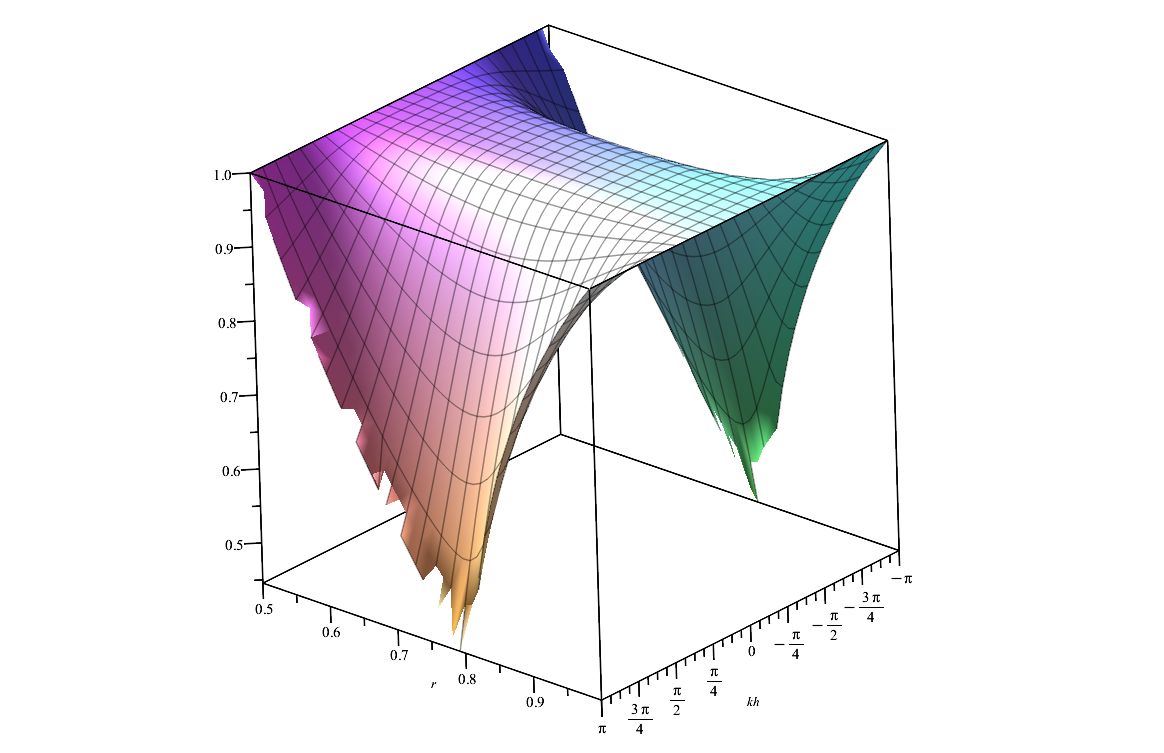
\includegraphics[width=0.6\linewidth]{dissipov1.png}}
\caption{Диссипативная поверхность для $\lambda_1$.}
\label{ris:dissipov1}
\end{figure}

\begin{figure}[h]
\center{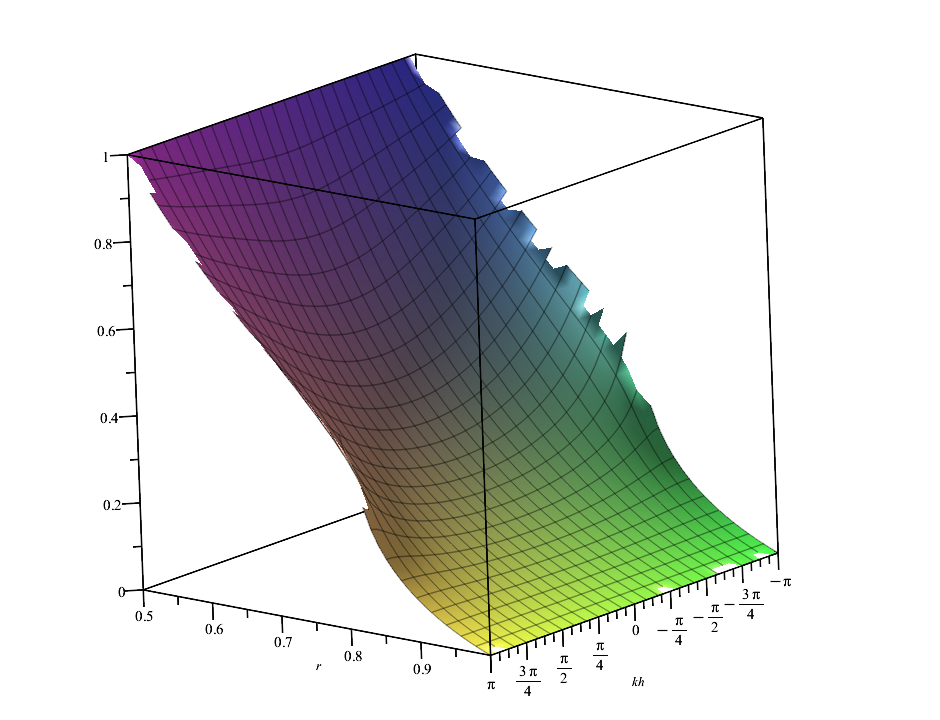
\includegraphics[width=0.6\linewidth]{dissipov2.png}}
\caption{Диссипативная поверхность для $\lambda_2$.}
\label{ris:dissipov2}
\end{figure}

\newpage Для дисперсионной поверхности воспользуемся соотношением $\lambda = e^{-i\omega \Delta t}$, а также тем, что $\omega = vk$.\\ 
Из этого следует, что $\frac{v}{c} = \frac{\omega}{ck} = \frac{-Arg(\lambda)}{ck\Delta t} = \frac{-Arg(\lambda)}{rk\Delta x}$.
\begin{figure}[h]
\center{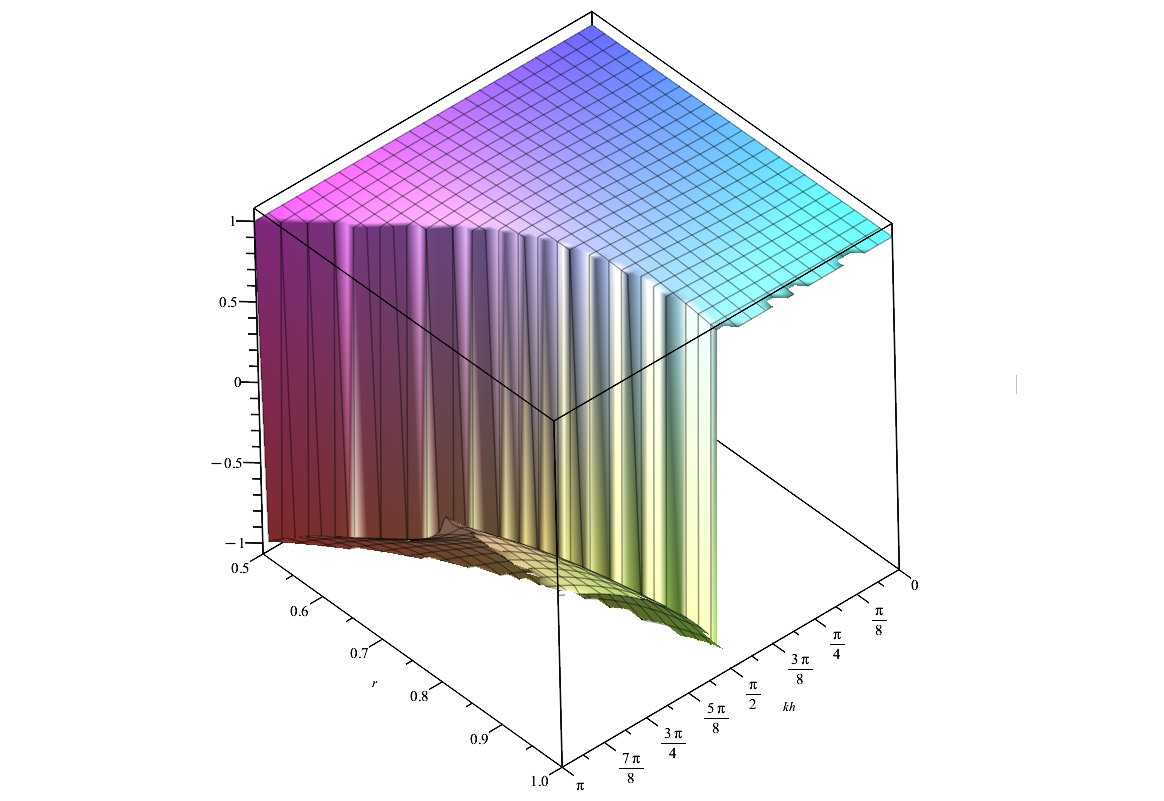
\includegraphics[width=0.6\linewidth]{dispepov1.png}}
\caption{Дисперсионная поверхность для $\lambda_1$.}
\label{ris:dispepov1}
\end{figure}

\begin{figure}[h]
\center{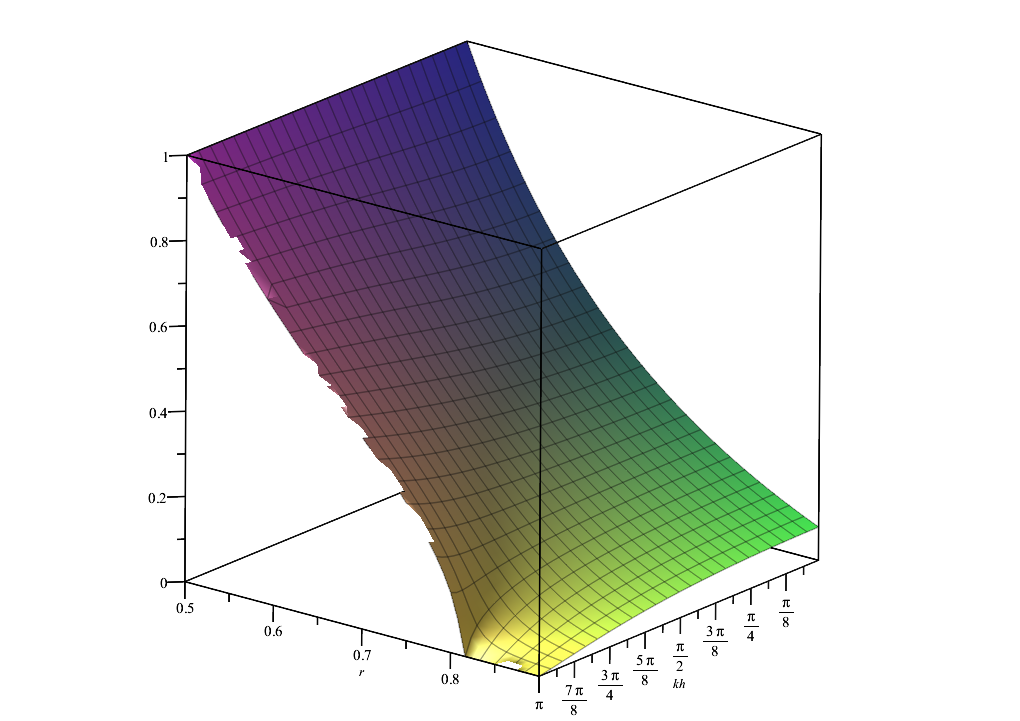
\includegraphics[width=0.6\linewidth]{dispepov2.png}}
\caption{Дисперсионная поверхность для $\lambda_2$.}
\label{ris:dispepov2}
\end{figure}

\par Дисперсионная поверхность для $\lambda_1$ представлена в интервале фазы от 0 до $\pi$, так как при отрицательном значении фазы Maple начинает выдавать неадекватные графики.





\newpage
\section*{Задание 6, 7}
\addcontentsline{toc}{section}{Задание 6, 7}
Проведите серию расчетов с самостоятельно подобранным набором на параметров для определения свойства схемы.\\
Проанализируйте и сравните результаты аналитического и численного исследования. Дайте характеристику схеме.
\par С использованием схемы были решены задачи со следующими начальными условиями:

\begin{figure}[h]
\center{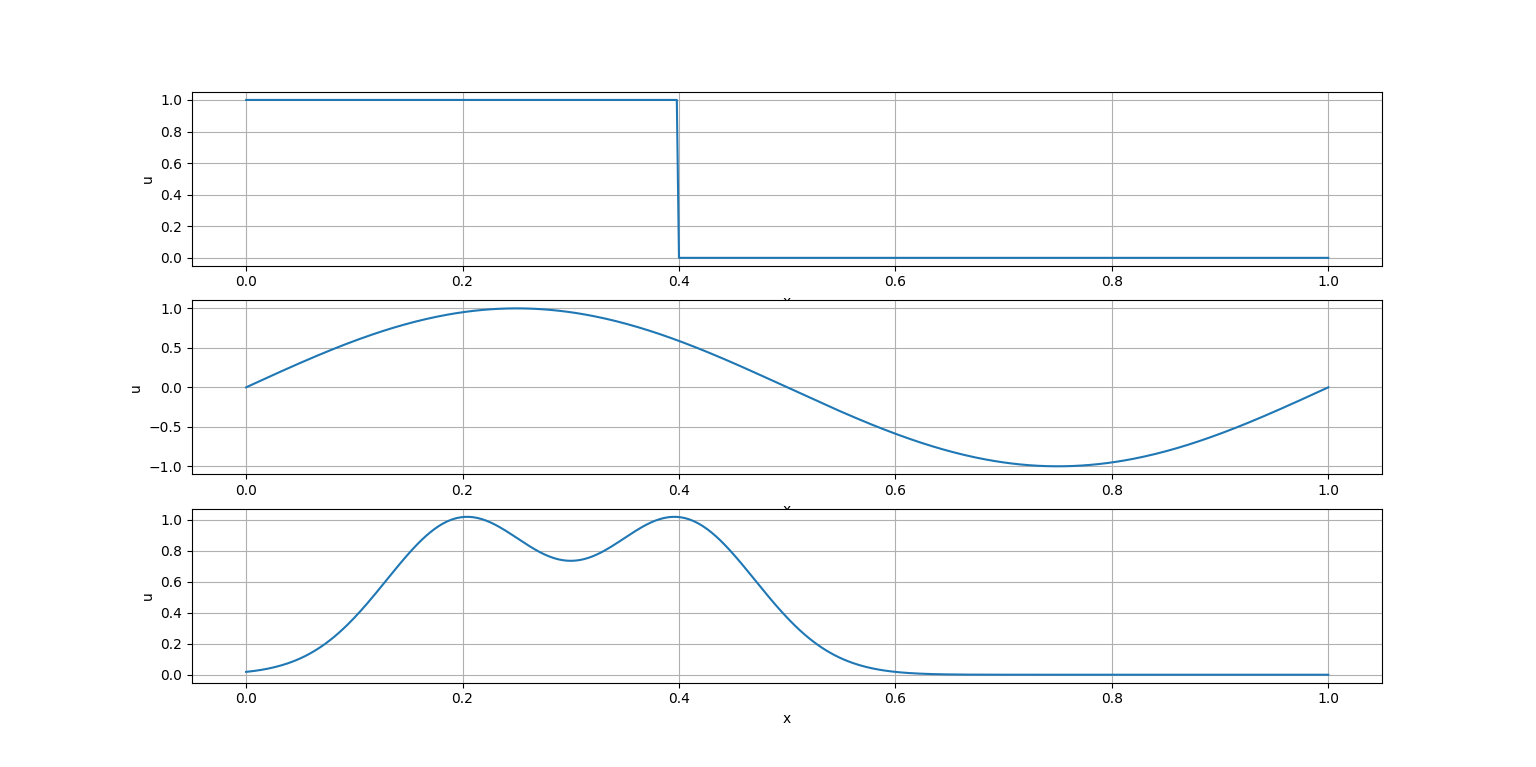
\includegraphics[width=0.85\linewidth]{initial_condition.png}}
\caption{Начальные условия.}
\label{ris:initial_condition}
\end{figure}

В результате работы программы были получены следующие графики:

\begin{figure}[h]
\center{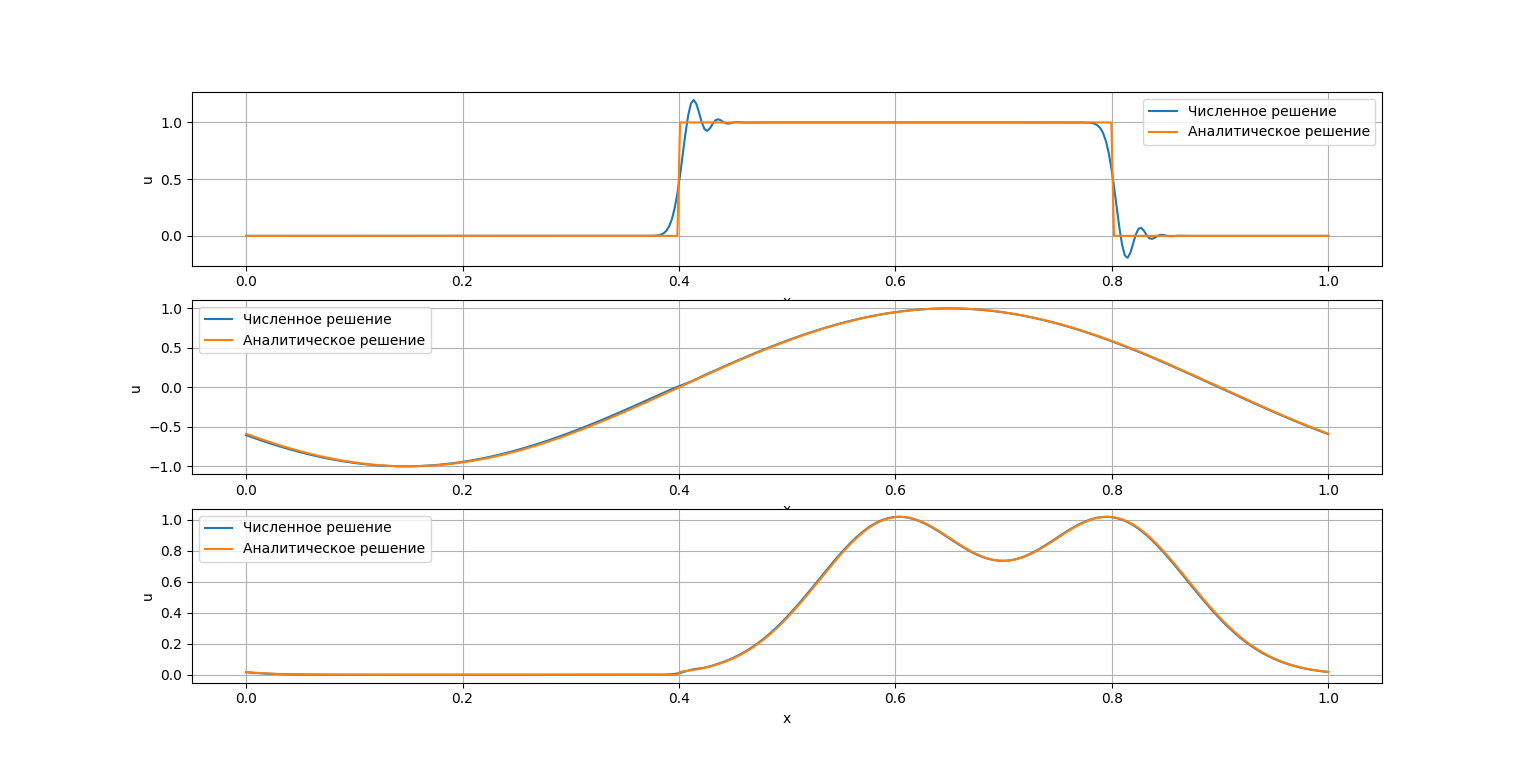
\includegraphics[width=0.85\linewidth]{final_conditionr08.png}}
\caption{Графики численных решений для $r=0.8$.}
\label{ris:final_conditionr08}
\end{figure}

\begin{figure}[h]
\center{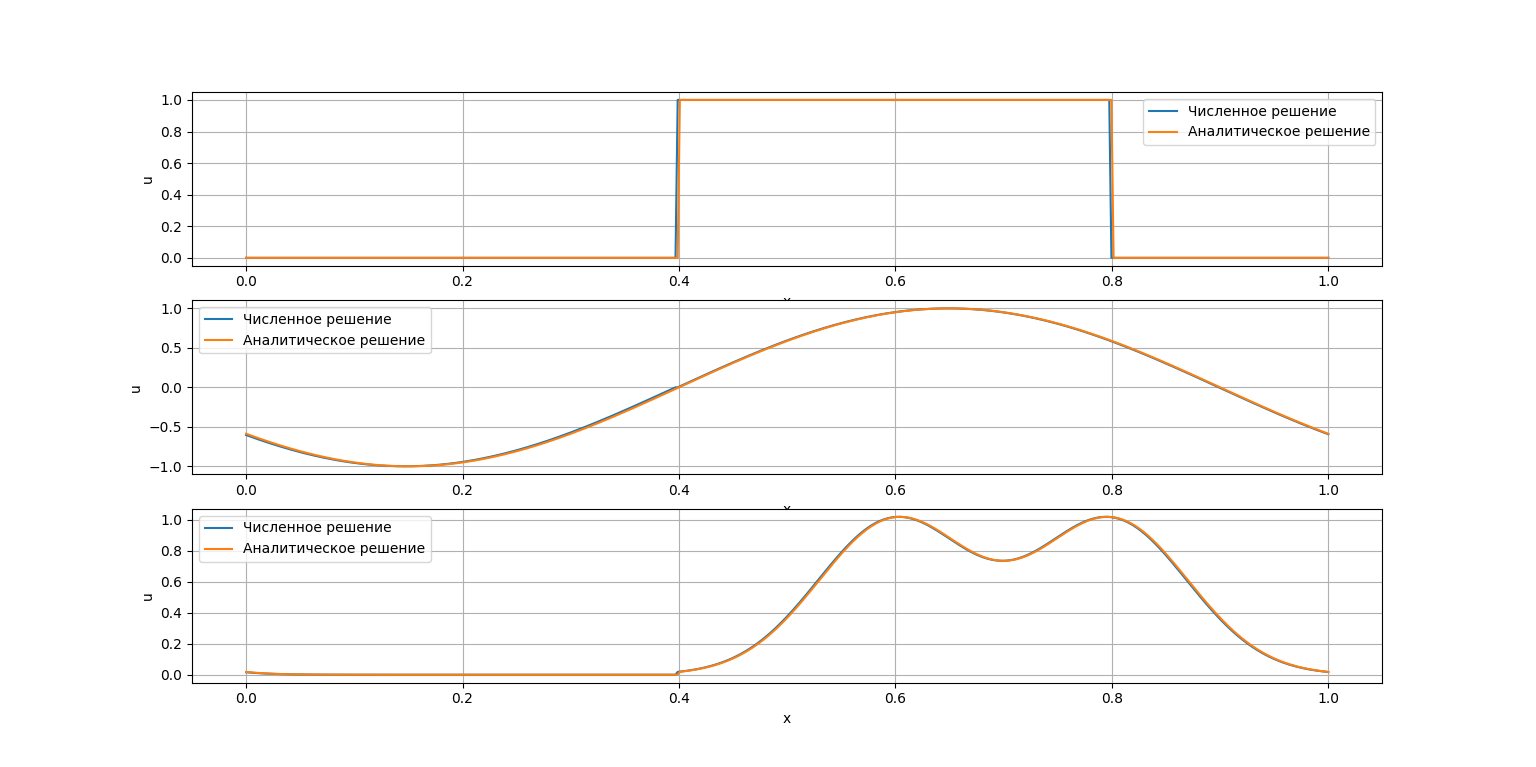
\includegraphics[width=0.85\linewidth]{final_conditionr1.png}}
\caption{Графики численных решений для $r=1$.}
\label{ris:final_conditionr1}
\end{figure}

\newpage Сравнивая аналитические и численные решения на графиках (\ref{ris:final_conditionr08}) и (\ref{ris:final_conditionr1}), можно сделать выводы о том, что схема является диссипативной (так как присутствует размытие ступеньки) и немонотонной (так как имеется дисперсия). Однако при $r = 1$ дисперсия и диссипация исчезают (что согласуется с графиком) и схема точно аппроксимирует решения.

\newpage
\section*{Задание 8}
\addcontentsline{toc}{section}{Задание 8}
С помощью метода неопределенных коэффициентов исследуйте шаблон, полученный на первом шаге, на свойство аппроксимации. Постройте график в пространстве неопределенных коэффициентов.\\

Формула для метода неопределенных коэффициентов согласно шаблону:
\begin{equation}
	\label{undef_coeff}
	\phi_{i+1}^{n+1} = a_{-1}\phi_{i-1}^{n+1}+a_0\phi_i^n+a_1\phi_i^{n-1}
\end{equation}

В результате разложения в ряд Тейлора и группировки соответствующих слагаемых была получена следующая система:
\begin{equation*}
	\begin{cases}
  	a_0+a_1+a_{-1} = 1
   	\\
   	-a_1+(r+1)a_{-1} = 1-r
   	\\
   	a_1+(r+1)^2a_{-1}=(1-r)^2
	\end{cases}
\end{equation*}

В результате решения системы были получены следующие значения для коэффициентов:
\begin{equation*}
	\begin{cases}
  	a_{-1} = \frac{r^2-3r+2}{r^2+3r+2}
   	\\\\
   	a_0 = \frac{-2r(r-2)}{r+1}
   	\\\\
   	a_1 = \frac{2r(r-1)}{r+2}
	\end{cases}
\end{equation*}

Также были построены графики в пространстве неопределенных коэффициентов $a_{-1}$ и $a_0$.
\begin{figure}[h]
\center{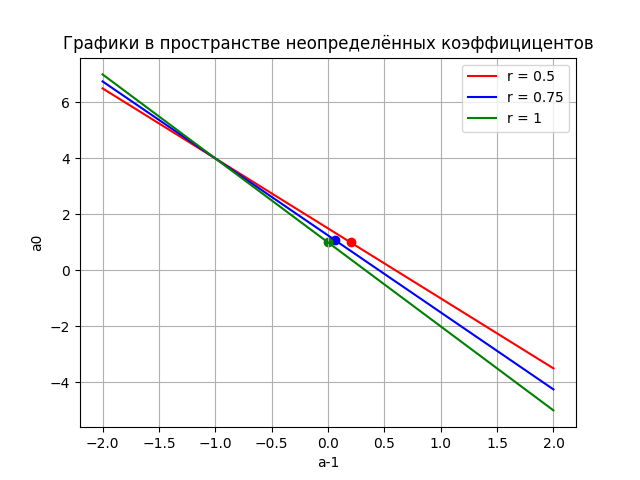
\includegraphics[width=0.65\linewidth]{undef_koeff_graph.png}}
\caption{Графики в пространстве неопределённых коэффициентов для разных чисел Куранта.}
\label{ris:undef_koeff_graph}
\end{figure}

\newpage
На рисунке (\ref{ris:undef_koeff_graph}) на прямых схема аппроксимирует уравнение переноса с первым порядком точности. В отмеченных точках у схемы второй порядок точности аппроксимации.

\newpage
\section*{Задание 9 (Заключение)}
\addcontentsline{toc}{section}{Задание 9 (Заключение)}
В ходе работы была исследована разностная схема, аппроксимирующая уравнение переноса. Было выяснено, что она аппроксимирует уравнение со вторым порядком точности по времени и по пространству. Схема является диссипативной и немонотонной, что было показано как с помощью прямых расчётов, так и с помощью диссипативных и дисперсионных поверхностей. 

\end{document}